\documentclass[11pt]{article}

\usepackage[margin=1in]{geometry}
\usepackage{amsmath,amssymb}
\usepackage{booktabs}
\usepackage{graphicx}
\usepackage{hyperref}

\newcommand{\plain}[1]{\medskip\noindent\fbox{\parbox{0.95\linewidth}{\textbf{In plain words.} #1}}\medskip}

\title{Why Accurate Models Are Easy to Fool:\\
A Hands-On Tour with a Toy Problem}
\author{}
\date{}

\begin{document}
\sloppy
\maketitle

\begin{abstract}
This paper is meant to be \emph{illustrative and tutorial}: a guided, hands-on way to understand the
possible culprits behind adversarial vulnerability, without needing specialist background. Image classifiers
can be fooled by changes too small for a person to notice. Why? We build the smallest problem we can where the
answer can be checked exactly: a task with one reliable clue and five unreliable clues, all of whose properties we
know. We train a small neural network on it, attack it, and take the problem apart one piece at a time, with each
section asking one plain question and answering it with a small experiment and a figure. What we find is simpler
than the usual stories. The network is fooled mainly because it adds up many small pieces of evidence, and an
attacker who may nudge every input a little can push all of them the same way. No single weak clue is to blame; their sum is.
We then show which fixes work and what they cost, when the effect appears and when it does not, and where the account holds up
and where it only partly holds on real images (circles and squares, MNIST, CIFAR-10). It is an aid to intuition, not a
claim about large deep networks in general.
\end{abstract}

\section{The idea in plain words}

A photo of a panda, plus a faint pattern of noise a person cannot see, is labelled ``gibbon'', with high confidence, by
a network that read the original correctly as ``panda'' (a famous example from Goodfellow et al.~\cite{goodfellow2015}). This is an \emph{adversarial example}.
Figure~\ref{fig:mnistadv} shows a real one from a small digit classifier: a handwritten digit it reads correctly with full confidence is turned into a different digit by changing
every pixel by at most $0.05$ or $0.06$ (on a scale where pixels span $1$), a change a person would barely notice.

\begin{figure}[h]
\centering
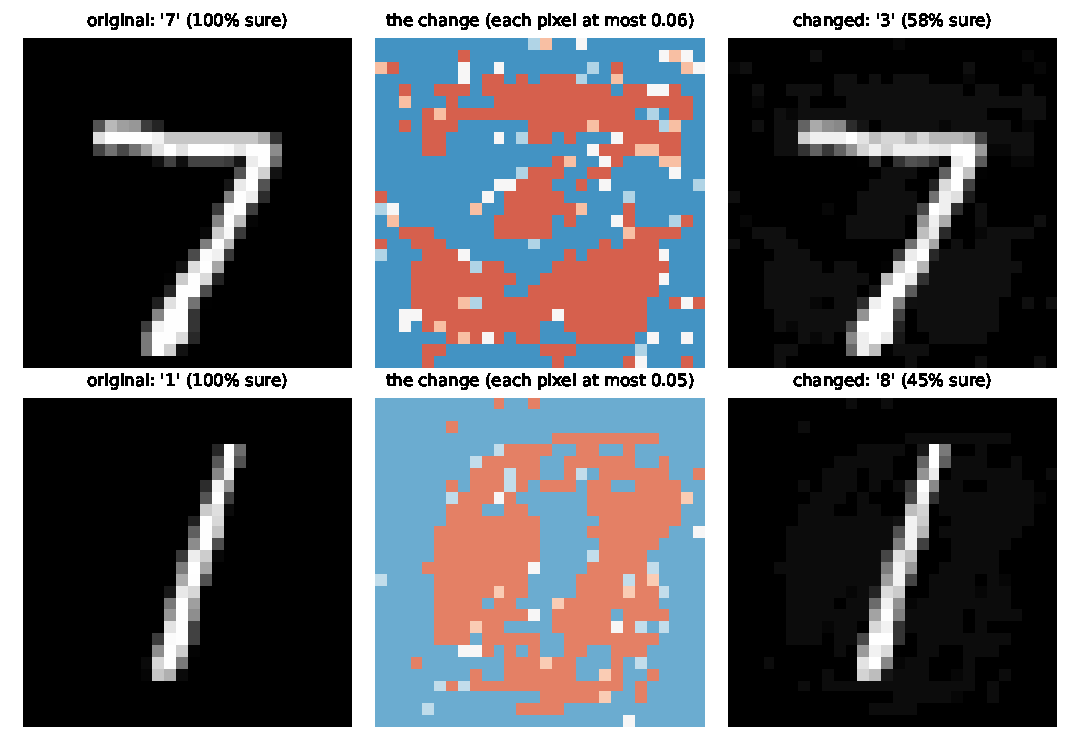
\includegraphics[width=0.78\textwidth]{fig_il_mnist_adv.pdf}
\caption{Two real adversarial examples from a small digit network. Left: the original digit and the network's answer. Middle: the change (red: brightened, blue: darkened; no pixel moves by more than the amount shown). Right: the changed digit and the network's new answer.}
\label{fig:mnistadv}
\end{figure}

Two explanations are often given:
\begin{itemize}
\item \textbf{Non-robust features} (Ilyas et al.~\cite{ilyas2019}). Images contain clues that
really do predict the label, but are fragile. A network trained to be accurate uses them, so it
inherits their fragility.
\item \textbf{Linearity in high dimension} (Goodfellow et al.~\cite{goodfellow2015}). A network
reads thousands of numbers. A tiny nudge to each of them, all in the unhelpful direction, adds up to
a big change in the answer.
\end{itemize}
These sound like rivals. In our toy world they turn out to be two views of one mechanism, and the
experiments below show which parts of each hold up.

\plain{Think of a vote among many voters. If the voters are independent, nudging one of them
does little. But an attacker who can whisper a tiny bias to \emph{every} voter at once can swing the
vote, even though no single voter was ever strongly persuaded.}

\paragraph{How to read this paper.} Each section poses a question, runs a small experiment, and
gives the answer in a box. Appendix~\ref{sec:glossary} is a short glossary. Numbers are averages over
10 random training runs (mean $\pm$ one standard deviation) unless stated; Appendix~\ref{app:details} gives the exact settings.

\paragraph{Where this sits.} Szegedy et al.~\cite{szegedy2014} first described adversarial examples; Goodfellow et al.~\cite{goodfellow2015}
introduced the one-step attack (FGSM) used here and Madry et al.~\cite{madry2018} its iterated version (PGD). Ilyas et al.~\cite{ilyas2019} proposed the
robust/non-robust decomposition we test, and Tsipras et al.~\cite{tsipras2018} argued robustness and accuracy can be at odds, which our trade-offs reproduce in
miniature. Athalye et al.~\cite{athalye2018} showed that many defenses fail once the attacker adapts, which is why we measure and do not propose a defense.

\section{A toy world}
\label{sec:world}

Every example is six numbers $x_0,\ldots,x_5$ and a label that is $0$ or $1$ with equal chance.

\begin{itemize}
\item $x_0$ is the \textbf{reliable clue}. Its average value is higher for label 1 than for label 0, with a
moderate amount of random wobble. Looking at $x_0$ alone and picking the nearer class gets the label right
$95\%$ of the time.
\item $x_1,\ldots,x_5$ are the \textbf{weak clues}. Each also shifts with the label, but the shift is small compared
with the wobble, so any one of them alone gets the label right only $79\%$ of the time.
\end{itemize}

Everything is known by construction, so we can compute, for any model, exactly how good it could possibly be.
The best possible classifier (called \emph{Bayes-optimal}) gets $99.3\%$. The wobble is bell-curve noise and the
numbers are not clipped to a range, which is what makes the best classifier a plain weighted sum of the six clues.

\begin{table}[h]
\centering
\caption{How good is each clue, and how good are they together? Accuracy of the best possible rule on each
set of clues (mean $\pm$ s.d.\ over 10 test sets).}
\label{tab:clues}
\begin{tabular}{lc}
\toprule
Clues used & Best possible accuracy \\
\midrule
reliable clue $x_0$ alone & $0.955\pm0.006$ \\
\emph{one} weak clue alone & $0.789\pm0.009$ \\
all five weak clues together & $0.963\pm0.009$ \\
all six clues & $0.993\pm0.002$ \\
\bottomrule
\end{tabular}
\end{table}

\plain{Five clues that are each only so-so are, together, \emph{better} than the one good clue. ``Weak'' does not
mean ``useless.'' It means weak one at a time.}

Figure~\ref{fig:clues} shows why. One weak clue alone (middle) barely separates the two classes. But the \emph{average} of the five weak clues (right) separates them
as well as the reliable clue does, because the wobble in independent clues partly cancels when they are averaged.

\begin{figure}[h]
\centering
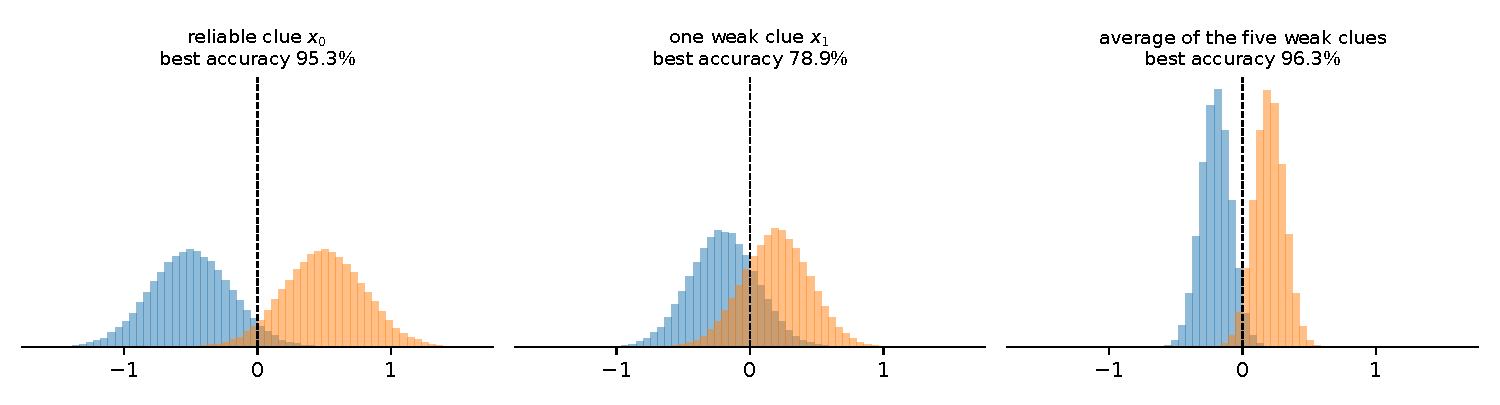
\includegraphics[width=\textwidth]{fig_il_clues.pdf}
\caption{The two classes (blue: label 0, orange: label 1) as seen through the reliable clue, one weak clue, and the average of the five weak clues. The dashed line is the best single threshold; the title gives the resulting accuracy.}
\label{fig:clues}
\end{figure}

\paragraph{Three models.} We train a tiny neural network (one hidden layer of 8 units) in three ways
(Figure~\ref{fig:arch}). \textbf{A} sees all six numbers. \textbf{B} sees only the reliable clue; the weak clues have no input at all.
\textbf{C} has input slots for all six but the weak ones are always set to zero.

\begin{figure}[h]
\centering
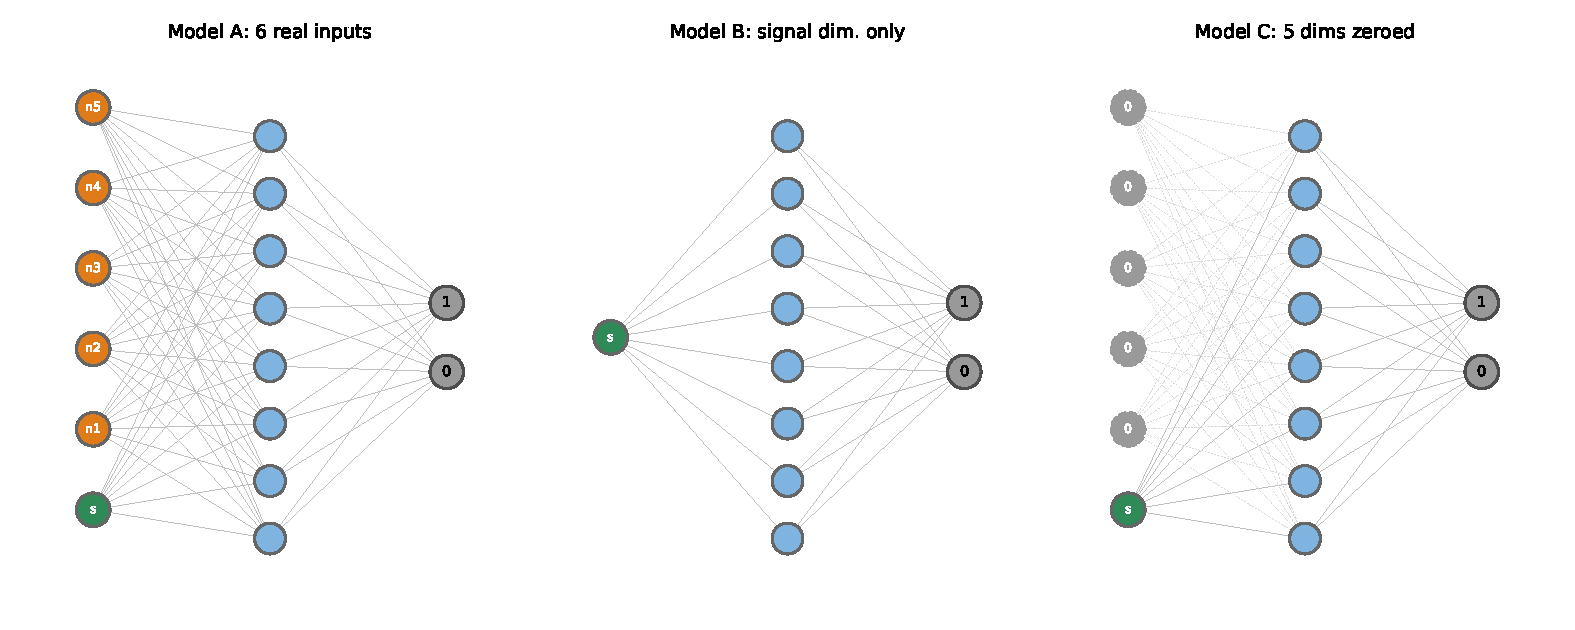
\includegraphics[width=0.9\textwidth]{fig_architectures.pdf}
\caption{The three models. Green: the reliable clue. Orange: the weak clues (only A sees their values).
Gray: slots that are always zero (C only).}
\label{fig:arch}
\end{figure}

\section{How we attack}

The attacker may change each input number by at most a small amount $\epsilon$ (we try $\epsilon$ up to $0.3$). The attacker chooses
the direction of each change to hurt the model most, using the model's own gradient (this is the standard one-step FGSM attack).
We count the share of correctly classified test points whose answer flips. We can also forbid the attacker from touching
some inputs, which lets us ask \emph{where} the model is vulnerable.

A nudge has to be judged against the \emph{size} of the clue it is applied to. Here the reliable clue's two class averages are $1.0$ apart (half-gap $0.5$)
and each weak clue's are $0.4$ apart (half-gap $0.2$), so a nudge of $0.3$ is already larger than a weak clue's half-gap. A very large nudge would make
anything look fragile; the sizes we use are chosen to be informative, not extreme.

\plain{The attack is not random noise. It is the worst possible nudge of a given size for the specific model.}

\paragraph{Is a one-step attack enough?} We also ran a stronger, iterated attack (PGD: 20 small steps from random starting points, 4 restarts) against
every model and subset of inputs. On the toy task it flips \emph{exactly} the same points as the one-step attack, at every nudge size and in every one of the 10 runs (the
largest per-run difference is $0.000$); for example $0.536$ against $0.536$ for all six inputs at $\epsilon=0.3$. The reason is that for this tiny network the direction
that hurts most does not change between the clean point and the edge of the allowed box, so there is nothing for extra steps to improve. This is a property of this small
network and task, not a general fact. On the image network of Section~\ref{sec:real} the iterated attack is stronger than the one-step attack.

\section{Question 1: who does the network listen to?}
\label{sec:listen}

The network (A) reaches $99.4\%$ accuracy, matching the best possible $99.3\%$. But does it use the weak clues the
way the best rule would? To compare fairly, we scramble one group of clues across the test set (so they stop carrying
information) and see how much accuracy drops. The bigger the drop, the more the rule depended on that group.

\begin{table}[h]
\centering
\caption{Accuracy lost when a group of clues is scrambled (mean $\pm$ s.d.\ over 10 runs).}
\label{tab:perm}
\begin{tabular}{lccc}
\toprule
 & reliable clue scrambled & weak clues scrambled & weak : reliable \\
\midrule
best possible rule & $0.213\pm0.009$ & $0.154\pm0.014$ & $0.72$ \\
trained network (A) & $0.245\pm0.011$ & $0.134\pm0.017$ & $0.55$ \\
\bottomrule
\end{tabular}
\end{table}

\plain{The network leans on the weak clues a bit \emph{less}, relative to the reliable one, than the best possible rule does. So the
common story, ``the network latches onto weak spurious clues too much,'' is not what is happening here. The weak clues are used about as
much as they deserve, and that is already enough to be exploited. The difference is modest, and we would not claim it holds for other
networks or training recipes.}

\begin{figure}[h]
\centering
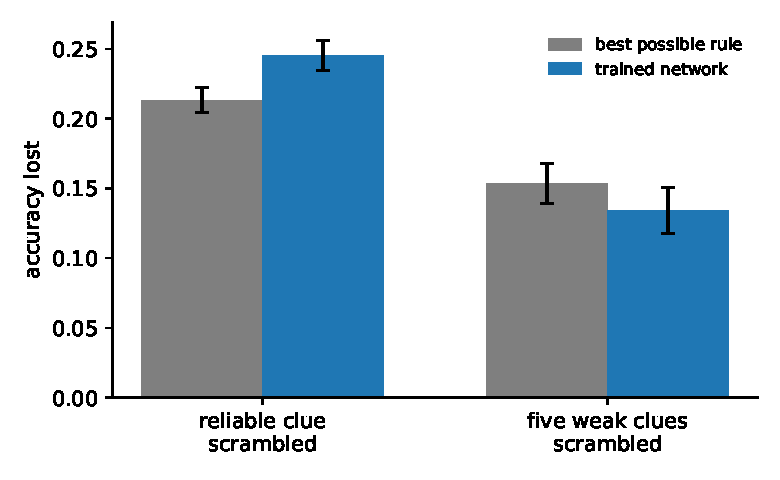
\includegraphics[width=0.58\textwidth]{fig_il_perm.pdf}
\caption{Accuracy lost when a group of clues is scrambled, for the best possible rule (gray) and the trained network (blue). Error bars: one standard deviation over 10 runs.}
\label{fig:perm}
\end{figure}

\section{Question 2: where is the network vulnerable?}
\label{sec:where}

We attack Model A while allowing the attacker to touch only some inputs.

\begin{table}[h]
\centering
\caption{Share of test points flipped at $\epsilon=0.3$ (mean $\pm$ s.d.\ over 10 runs). Clean accuracy: A $0.994$,
B $0.956$, C $0.956$.}
\label{tab:attack}
\begin{tabular}{lc}
\toprule
What the attacker may change & Flipped \\
\midrule
all six inputs (Model A) & $0.536\pm0.020$ \\
the reliable clue only & $0.037\pm0.005$ \\
all five weak clues & $0.260\pm0.014$ \\
\emph{just one} weak clue & $0.012\pm0.003$ \\
\midrule
Model B (reliable clue only), attacker may change it & $0.211\pm0.014$ \\
\bottomrule
\end{tabular}
\end{table}

\begin{figure}[h]
\centering
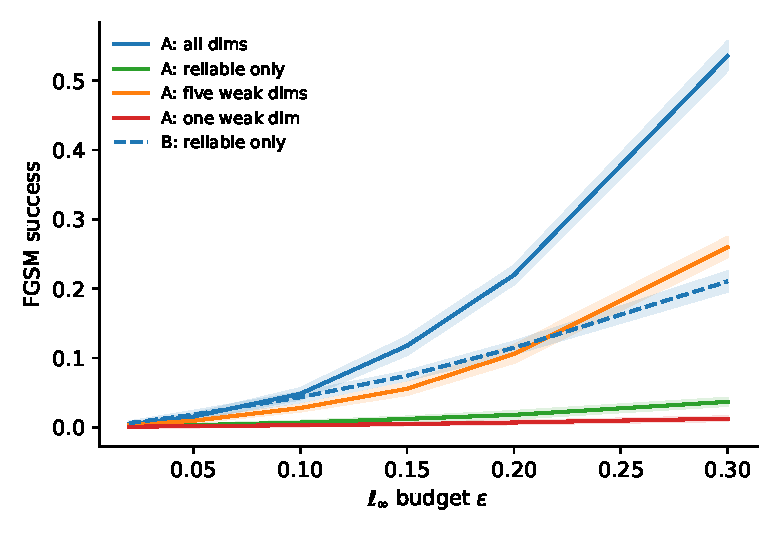
\includegraphics[width=0.62\textwidth]{fig_fr_curves.pdf}
\caption{Share flipped against attack size $\epsilon$. One weak clue (red) is the hardest thing to exploit; five together (orange) are
far easier than the reliable clue alone (green).}
\label{fig:curves}
\end{figure}

The first reading of the table is tempting: attacking the five weak clues is several times as effective as attacking the reliable one
($0.26$ against $0.04$), so \emph{the weak clues are the weak spot}. The row ``just one weak clue'' shows why that is misleading. A single weak
clue flips only $1.2\%$, \emph{less} than the reliable one. The first comparison was five coordinates against one, not weak against strong.

Figure~\ref{fig:nudges} shows the mechanism on one test point. Each weak clue, nudged by $0.3$, takes a little off the network's
confidence. Nudging only the reliable clue leaves the point correctly classified. After four weak nudges the answer flips.

Averaged over all test points and runs, the same story appears in Figure~\ref{fig:kdims}: the share flipped climbs steadily as the attacker is allowed to touch one, two, \ldots, five weak clues, and each added clue adds more than the one before.

\begin{figure}[h]
\centering
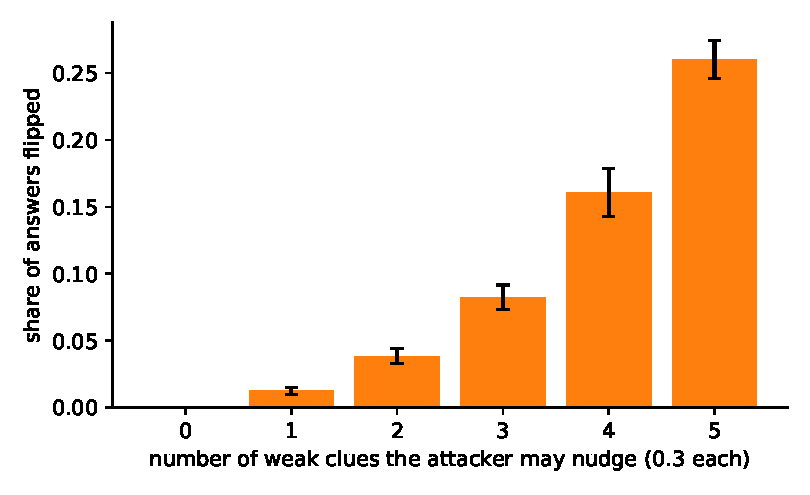
\includegraphics[width=0.58\textwidth]{fig_il_kdims.pdf}
\caption{Share of answers flipped (Model A, nudge $0.3$) as the attacker may nudge more and more of the weak clues. The reliable clue is never touched. Error bars: one standard deviation over 10 runs.}
\label{fig:kdims}
\end{figure}

\begin{figure}[h]
\centering
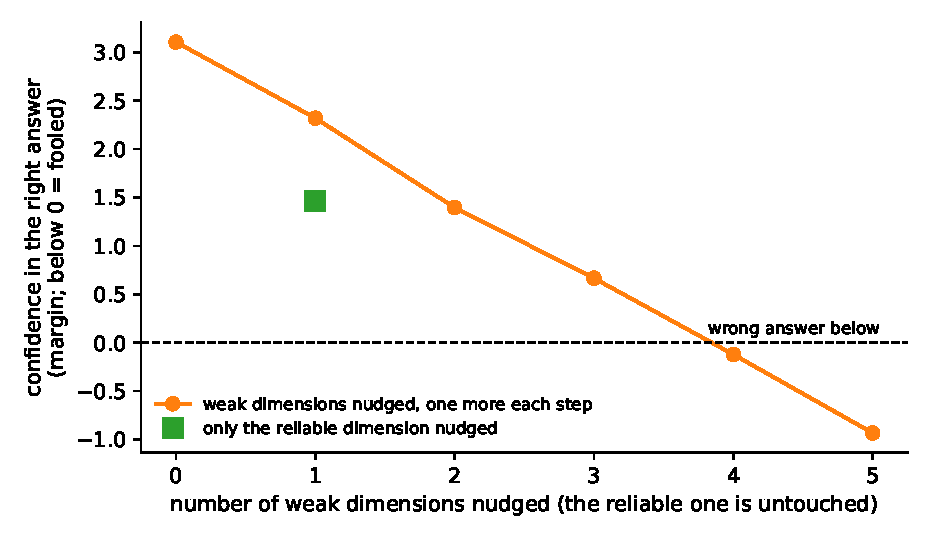
\includegraphics[width=0.7\textwidth]{fig_il_nudges.pdf}
\caption{One test point (Model A; a typical point among those where nudging the reliable clue alone does not flip it). Orange: the model's
confidence in the right answer as more weak clues are nudged by $0.3$, one more at each step; the answer flips at four. Green: nudging
the reliable clue alone. Below the dashed line the model is fooled.}
\label{fig:nudges}
\end{figure}

Two more views of the same fact (one training run each). Figure~\ref{fig:slices} slices the network's decision along each input in turn: the reliable clue
gives a steep, well-separated curve, each weak clue a shallow ramp. A shallow ramp per clue is exactly why one weak nudge does little; five of them add up. Figure~\ref{fig:example}
shows one real attack: with the reliable clue untouched, the combined shift in five weak clues alone flips the answer.

\begin{figure}[h]
\centering
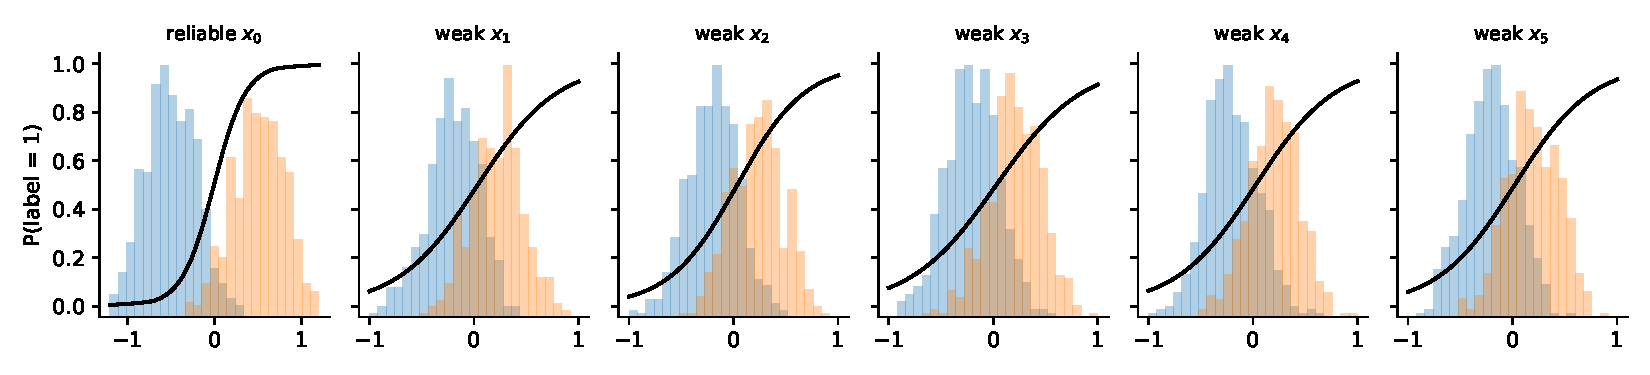
\includegraphics[width=\textwidth]{fig_il_slices.pdf}
\caption{One training run. The network's predicted probability of label 1 (black) as each input is varied alone (others held at their average), with the two classes' distributions behind (blue: label 0, orange: label 1).}
\label{fig:slices}
\end{figure}

\begin{figure}[h]
\centering
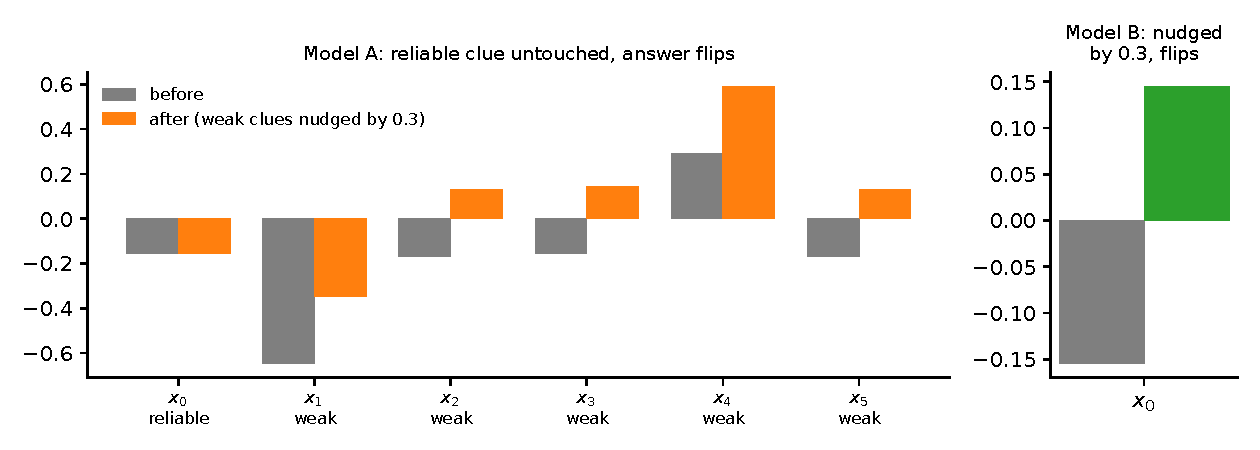
\includegraphics[width=0.85\textwidth]{fig_il_example.pdf}
\caption{One successful attack per model at $\epsilon=0.3$ on one test point, one training run. Left: attack allowed only on the weak clues; the reliable clue is unchanged yet the
answer flips. Right: the model that sees only the reliable clue, attacked directly.}
\label{fig:example}
\end{figure}

Figure~\ref{fig:subsets} repeats the comparison in terms of \emph{flip size}, the smallest nudge needed, which is easier to interpret than a share: attacking the reliable clue alone needs a nudge of about $1.1$;
attacking one weak clue needs $1.9$ (harder); attacking all five weak clues needs $0.37$ (much easier); attacking everything needs $0.28$. The exact best rule and the trained network agree.

\begin{figure}[h]
\centering
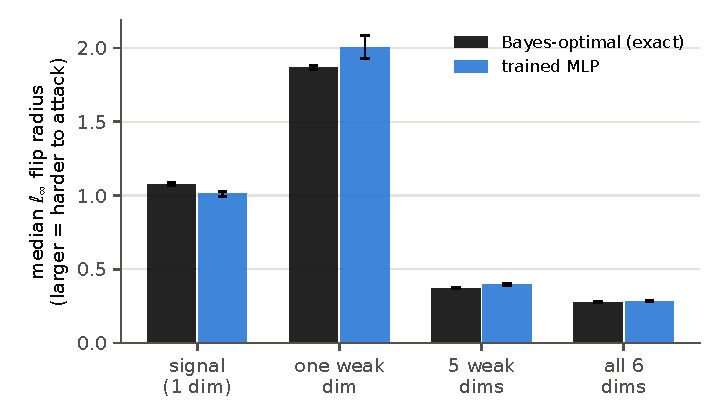
\includegraphics[width=0.62\textwidth]{fig_rc_subsets.pdf}
\caption{Median flip size (the smallest nudge that flips a point; larger means harder to attack) when the attacker controls only the listed inputs. Black: exact best rule. Blue: trained network (mean $\pm$ s.d.\ over 10 runs).}
\label{fig:subsets}
\end{figure}

\plain{No single weak clue is fragile. The weak clues are dangerous \emph{together}, because their small effects pile up when the attacker pushes them
all the same way. ``Attacks through the weak features work better'' is true only because there are five of them.}

\section{Question 3: why does adding up make things fragile?}
\label{sec:why}

When the best rule is a weighted sum $\sum_i w_ix_i$, the smallest change per input that flips an answer is
\[
\text{flip size}=\frac{\text{how confident the sum is}}{\sum_i |w_i|}.
\]
Each input contributes its own $|w_i|$ to the denominator, so \emph{more inputs carrying the evidence means a smaller flip size}.
This quantity, the sum of absolute weights $\|w\|_1$, is the whole story for a weighted sum: it is how far the answer moves when
every input is nudged by one unit in the worst direction. In our task the reliable clue has weight $11.1$ and each weak clue $6.4$,
so the five weak clues together carry $32.0$, nearly three times as much.

\begin{figure}[h]
\centering
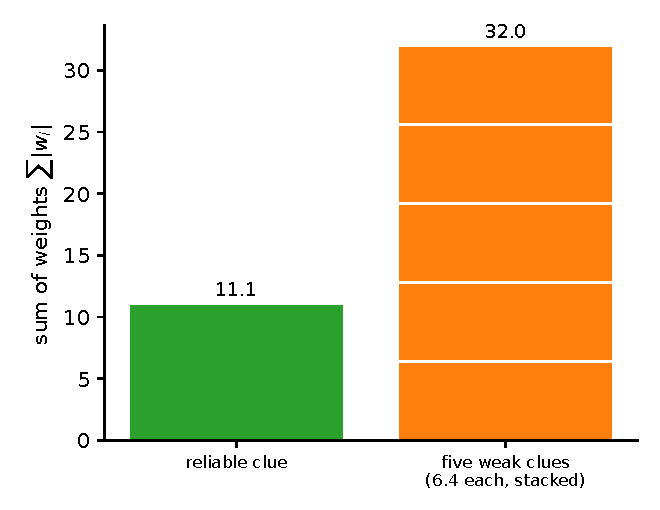
\includegraphics[width=0.46\textwidth]{fig_il_weights.pdf}
\caption{The sum of weights $\sum|w_i|$, which sets how far a full nudge moves the answer. One reliable clue carries $11.1$; the five weak clues, stacked, carry $32.0$.}
\label{fig:weights}
\end{figure}

A picture helps (Figure~\ref{fig:geometry}). Draw the allowed changes for two inputs as a square (each input may move by at most $\epsilon$) and the decision boundary as a line. If all the evidence is in one input, the boundary is a vertical line and the
square must grow until its \emph{side} reaches it. If the same evidence is split over two inputs, the boundary is diagonal, and the square's \emph{corner}, which moves both inputs at once, reaches it sooner. The straight-line distance to the boundary (blue circle) is the same in both cases;
only the square, the per-input change, shrinks, by $1/\sqrt2$ here and by $1/\sqrt k$ for $k$ inputs.

\begin{figure}[h]
\centering
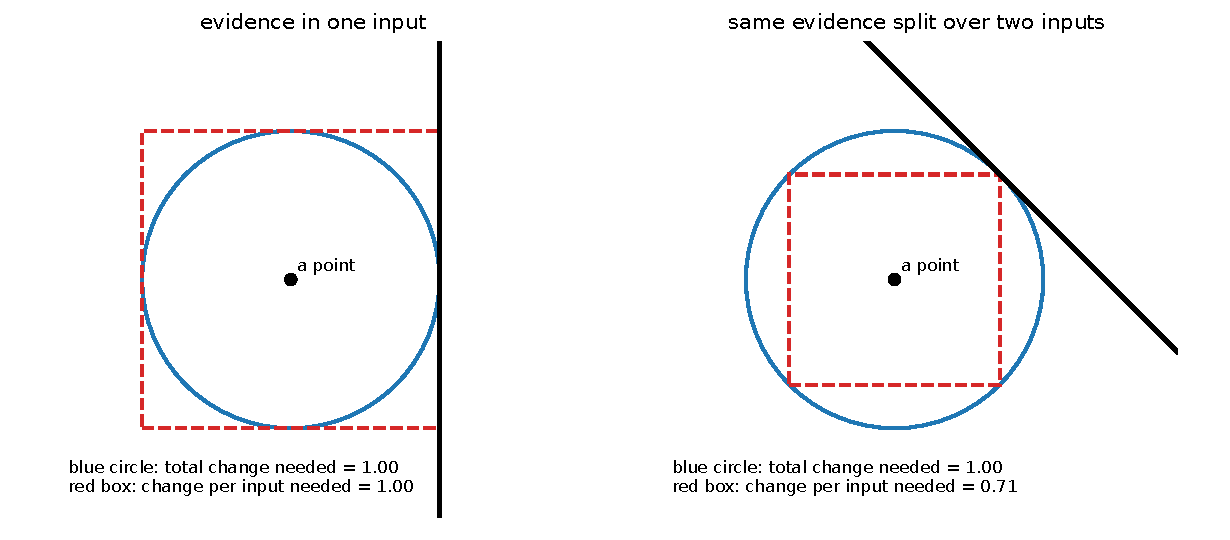
\includegraphics[width=0.9\textwidth]{fig_il_geometry.pdf}
\caption{Two inputs, one point. Blue circle: total change needed to reach the decision boundary (black). Red dashed square: per-input change needed. Splitting the evidence over two inputs leaves the circle unchanged and shrinks the square.}
\label{fig:geometry}
\end{figure}

\subsection{The same evidence, spread out}

To test this directly we keep the total amount of evidence fixed and split it equally over $k$ inputs, $k=1,2,4,\ldots,64$. A classifier
with the same accuracy ($95\%$) is built each time.

\begin{figure}[h]
\centering
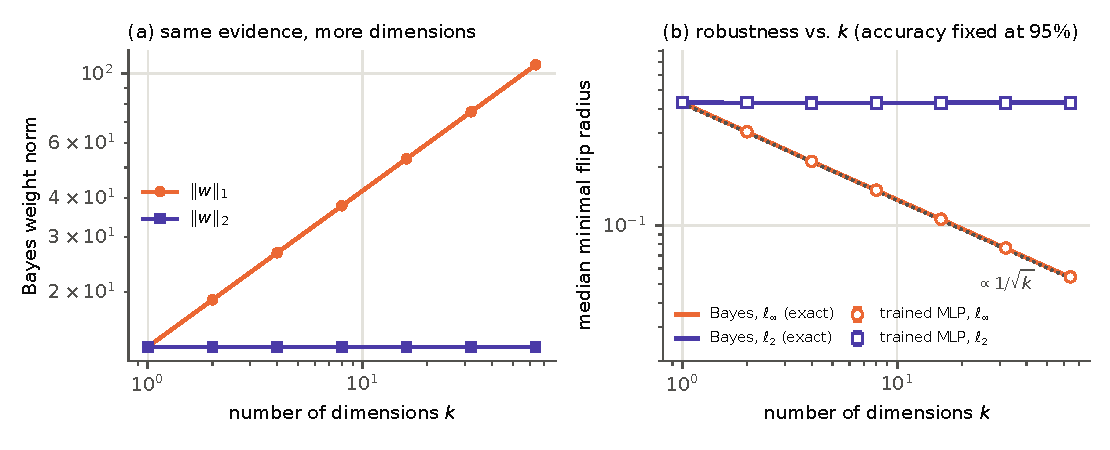
\includegraphics[width=0.98\textwidth]{fig_rc_dimensions.pdf}
\caption{Spreading a fixed amount of evidence over more inputs. Right panel: the smallest per-input change that flips an answer
(median) falls as $1/\sqrt k$ (steep lines) while the \emph{total size} of the change needed (the $\ell_2$ distance, flat lines) stays put.
Exact best rule (lines) and trained networks (markers) coincide.}
\label{fig:spread}
\end{figure}

With $k=1$ the per-input flip size is $0.43$; with $k=64$ it is $0.054$, eight times smaller, at the same accuracy. Measured the other way,
as the total size of the change (the ordinary straight-line distance), nothing changes: $0.43$ throughout. The trained network follows the exact curve at every $k$.

\plain{Splitting the same information over more inputs makes the model eight times easier to fool when each input may be nudged a little,
without making it less accurate and without making any individual input more fragile. If instead the attacker is limited by the
\emph{total} size of the change, there is no difference.}

\subsection{A property of the problem, not of the network}

We can also attack the \emph{best possible} classifier, which involves no training at all. It is just as vulnerable as the trained one:
the median per-input flip size is $0.277$ for the best rule and $0.285$ for the network.

\begin{figure}[h]
\centering
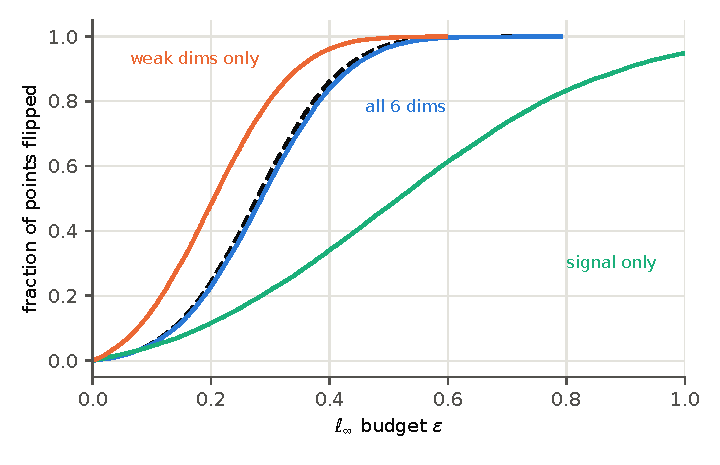
\includegraphics[width=0.58\textwidth]{fig_rc_ecdf.pdf}
\caption{Share of test points flipped as the allowed nudge grows. The best possible rule (dashed black) lies on top of the trained network (blue). Networks that see only the five weak clues (orange) or only the reliable clue (green) are shown for comparison.}
\label{fig:ecdf}
\end{figure}

\plain{The network is not doing something silly that a better training run would avoid. The fragility belongs to the problem and to the
kind of attack allowed.}

\subsection{Small clues, not unreliable clues}

``Weak'' has so far meant ``unreliable.'' But the notion of ``non-robust'' in the original theory is about a clue being \emph{small} relative to the
nudge, not unreliable. To separate the two, we took a single clue and varied them independently: its \emph{size} (the gap between the two
class averages) and its \emph{reliability} (how well it predicts the label).

\begin{figure}[h]
\centering
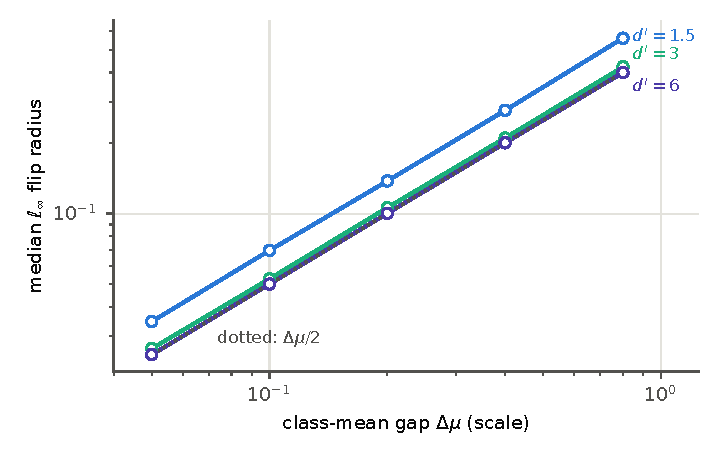
\includegraphics[width=0.58\textwidth]{fig_rc_scale.pdf}
\caption{Flip size of a single-clue classifier against the clue's size (class gap), at three reliabilities (log scales). The lines are almost on top of one another: size matters, reliability hardly does. Lines: exact; markers: trained network.}
\label{fig:scale}
\end{figure}

\begin{table}[h]
\centering
\caption{Smallest per-input change that flips a single-clue classifier (median). Rows: clue size; columns: how reliable the
clue is (accuracy: 77\%, 93\%, 99.9\%).}
\label{tab:scale}
\begin{tabular}{lccc}
\toprule
Size of the clue & 77\% reliable & 93\% reliable & 99.9\% reliable \\
\midrule
0.05 & 0.035 & 0.027 & 0.025 \\
0.2  & 0.138 & 0.106 & 0.100 \\
0.8  & 0.560 & 0.422 & 0.400 \\
\bottomrule
\end{tabular}
\end{table}

\plain{The flip size is proportional to the clue's \emph{size}: shrink the clue sixteenfold and the flip size shrinks sixteenfold. Making the clue
more reliable does not make it safer; if anything, a nearly perfectly reliable clue is slightly \emph{easier} to flip, because with one clue the flip
size is just the distance to the decision boundary, and a very reliable clue puts almost every point about half the class gap from it, while a less reliable
clue leaves some points farther away. A tiny clue that is 99.9\% reliable can be flipped by a nudge of $0.025$.}

\section{Question 4: can we fix it?}
\label{sec:fix}

\paragraph{Remove the weak clues.} Model B, which never sees them, is much harder to fool at large nudge sizes: $0.211$ flipped at $\epsilon=0.3$ against
$0.536$ for A. The price is $3.8$ points of accuracy ($99.4\%\to95.6\%$). Below $\epsilon=0.10$ there is no visible gain. This is a trade, not a free fix:
the weak clues really did carry information.

\paragraph{Freezing the weak clues at zero (Model C).} A cheaper idea than removing the inputs is to keep the slots but always feed zeros. The slots are
then never trained, and one might worry that an attacker could use their leftover random weights. In practice not: with ordinary initialisation, nudging those slots flips $0\%$ of points
(in all 10 runs), and Model C behaves exactly like Model B ($0.211$ flipped at $\epsilon=0.3$ for both). But this safety is about \emph{size}: if we multiply the leftover weights by $3$ or $10$ it stays
at $\approx0$ ($0.000$ and $0.001\pm0.001$), and at $100\times$ it collapses ($0.92\pm0.12$ flipped). For a single layer the reason is exact: the worst-case shift is the nudge size times the sum of those weights'
absolute values, so safety lasts only while that product stays below the model's confidence.

\begin{figure}[h]
\centering
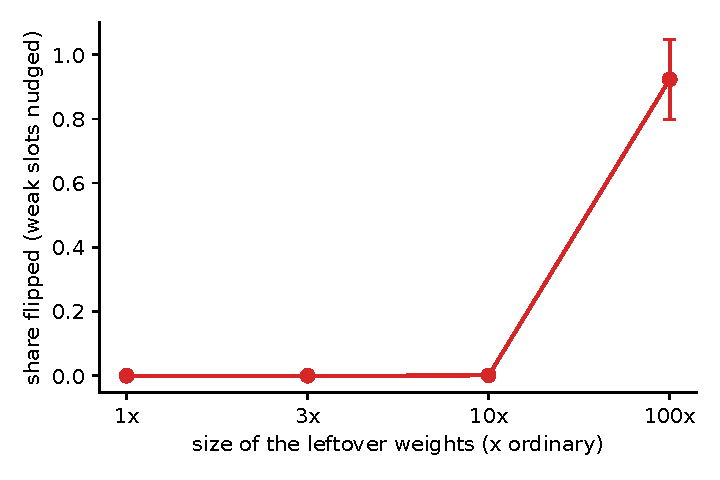
\includegraphics[width=0.52\textwidth]{fig_il_modelc.pdf}
\caption{Model C: share flipped when the attacker nudges only the frozen weak slots, as their leftover weights are multiplied by $1$, $3$, $10$ and $100$ (10 runs).}
\label{fig:modelc}
\end{figure}

\paragraph{Let the model remove them itself.} Instead of deciding in advance which clue is reliable, we can penalise the model for using many inputs.
Penalties that switch whole inputs off (the $L_1$ penalty, group Lasso, elastic net) behave like Model B without being told which clue to keep.

\begin{table}[h]
\centering
\caption{Attack on the five weak clues at $\epsilon=0.3$ (mean $\pm$ s.d.\ over 10 runs). Baseline: ordinary training. Each trained-penalty row is a setting with accuracy close to $0.97$; the last row is ordinary shrinkage at its strongest setting that still works.}
\label{tab:reg}
\begin{tabular}{lcc}
\toprule
Training recipe & Accuracy & Flipped \\
\midrule
baseline & $0.994\pm0.003$ & $0.260\pm0.014$ \\
$L_1$ penalty & $0.969\pm0.005$ & $0.023\pm0.008$ \\
group Lasso & $0.975\pm0.005$ & $0.038\pm0.012$ \\
elastic net & $0.979\pm0.004$ & $0.050\pm0.008$ \\
simply deleting 4 weak inputs afterwards & $0.970\pm0.005$ & $0.052\pm0.007$ \\
ordinary shrinkage ($L_2$), strength 0.2 & $0.993\pm0.003$ & $0.213\pm0.013$ \\
\bottomrule
\end{tabular}
\end{table}

Ordinary shrinkage ($L_2$, the standard ``weight decay'') cannot reach that regime: with moderate strength it costs no accuracy and helps a little; at strength $0.4$ it
collapses to chance, with nothing in between.

Figure~\ref{fig:frontier} shows every setting we tried at once. The selective penalties and deleting inputs trace a smooth curve from ``accurate but easy to fool'' to ``a bit less accurate but hard to fool''. Ordinary shrinkage ($L_2$, red crosses) sits on the accurate end of the same curve and
then falls off a cliff.

\begin{figure}[h]
\centering
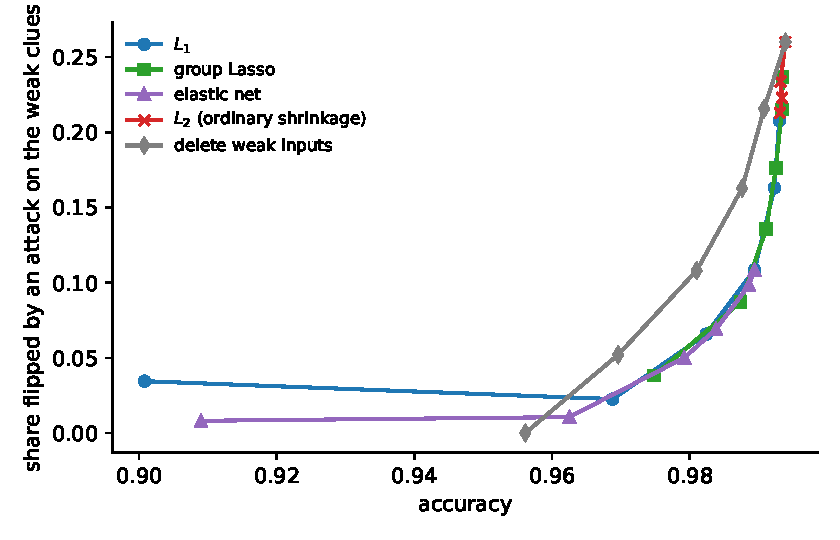
\includegraphics[width=0.66\textwidth]{fig_il_frontier.pdf}
\caption{Accuracy against the share flipped by an attack on the weak clues, for every setting of each method (mean over 10 runs). Lower and further right is better. The point at the far left of the $L_1$ line (strongest penalty) has runs that over-shrink the reliable clue.}
\label{fig:frontier}
\end{figure}

\begin{figure}[h]
\centering
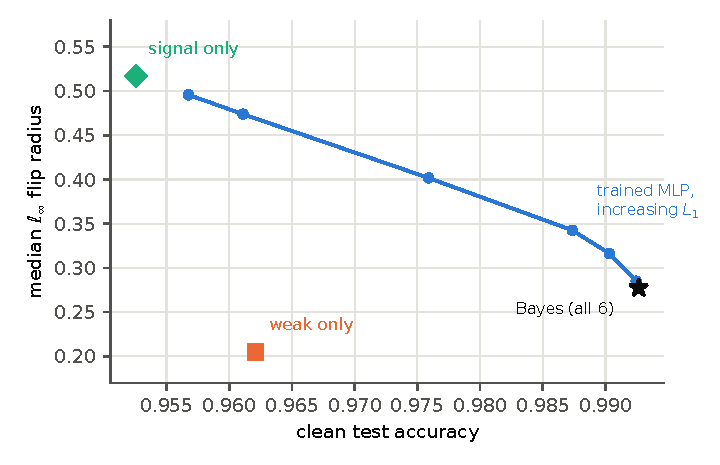
\includegraphics[width=0.6\textwidth]{fig_rc_tradeoff.pdf}
\caption{Accuracy against robustness. As the $L_1$ penalty grows (blue), the model moves from the best possible point (star) toward the
reliable-clue-only model (green). The weak-only model (orange) is more accurate than reliable-only but far less robust.}
\label{fig:tradeoff}
\end{figure}

\paragraph{The cost of concentrating.} Putting all the weight on the reliable clue has a downside. With the $L_1$ penalty the weak-clue attack falls from $0.260$ to $0.023$, but an attack on the reliable clue alone
rises from $0.037$ to $0.173$ (and Model B, which has only that clue, sits at $0.211$). With the redundancy gone, the one clue left is a bigger single point of failure. The net effect is still a large win, because the weak-clue loss is
so much bigger, but the trade-off exists whether the removal is done by us or by the penalty.

\paragraph{Choosing the penalty strength.} A very light $L_1$ penalty can look like it does nothing if it is compared against the wrong baseline: the weight on the reliable clue relative to the weak ones is $2.4$ at strength $0.02$ against $2.0$ for
ordinary training, an unremarkable change. Sweeping the strength shows the ratio climbing from $2.4$ to $18$ (at $0.4$) while accuracy slips only from $99.3\%$ to $96.9\%$ (Figure~\ref{fig:l1sweep}).
Pushed too far ($0.8$), some runs over-shrink even the reliable clue and fall apart (mean accuracy $0.90\pm0.15$). The practical lesson is to compare against a true no-penalty baseline, and to sweep.

\begin{figure}[h]
\centering
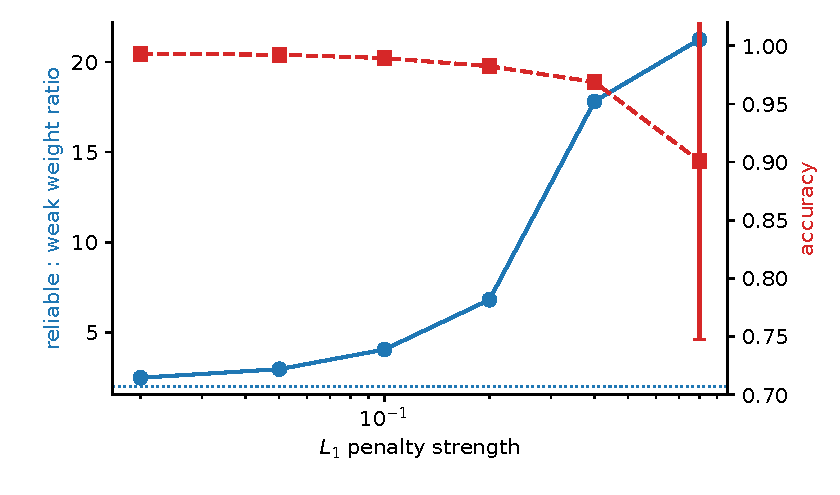
\includegraphics[width=0.6\textwidth]{fig_il_l1sweep.pdf}
\caption{Effect of the $L_1$ penalty strength (10 runs per point). Blue: ratio of the weight on the reliable clue to the weight on the weak clues (median over runs; dotted line: ordinary training). Red: accuracy, mean $\pm$ s.d.
The ratio rises from about $2$ to about $18$ while accuracy slips mildly; at the strongest value some runs over-shrink the reliable clue itself, which is why the error bar is so wide.}
\label{fig:l1sweep}
\end{figure}

\paragraph{Not every kind of sparsity helps.} A different standard penalty discourages \emph{hidden activity} (how many internal units fire) instead of how large the input weights are. It does what it is meant to: the average
activity falls from $0.42$ to $0.07$ and the fraction of silent units rises from $38\%$ to $93\%$. But it has no handle on \emph{which input} to keep: the reliable-to-weak weight ratio stays flat ($1.97\to1.81$), and the
weak-clue attack is as effective as ever ($0.260$ against $0.255$--$0.276$ at every strength up to $2.0$). Pushed harder, it fails abruptly instead of gradually: each run either stays fully accurate or becomes a dead network at chance
(Figure~\ref{fig:actsparse}); no run was ever in between. The number of dead runs rises with strength ($0$ of $10$ up to $2.0$, $2$ at $3.0$, $7$ at $4.0$, $9$ at $6.0$, all $10$ at $8.0$), so the \emph{average} accuracy appears to decline smoothly although no single network ever does.
A single run would therefore either miss the collapse or mistake it for typical. (We tested one such penalty on this one network; we do not claim it holds for other forms of activation sparsity.)

\begin{figure}[h]
\centering
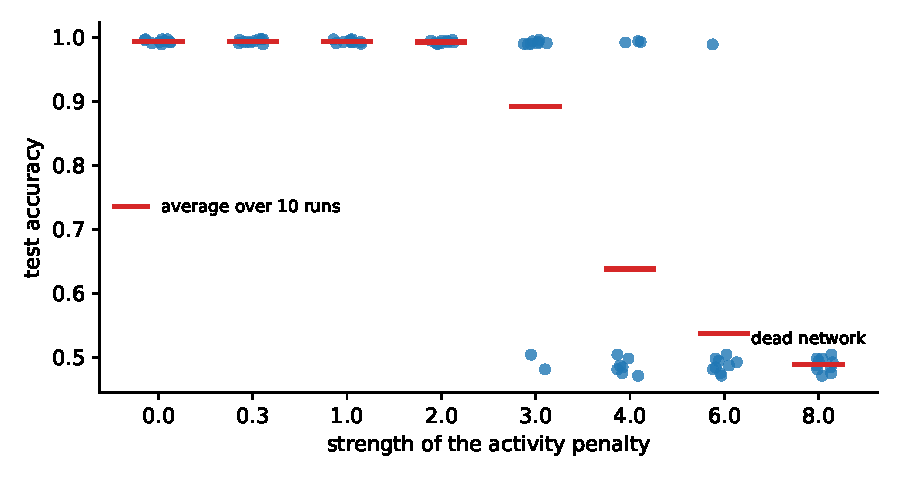
\includegraphics[width=0.66\textwidth]{fig_il_actsparse.pdf}
\caption{Each dot is one training run (10 per strength). Accuracy is all-or-nothing: functional runs stay near $99\%$, dead networks sit at chance. The red bar, the average, falls smoothly only because the share of dead runs grows.}
\label{fig:actsparse}
\end{figure}

\plain{Every fix that works does the same thing: it reduces the sum of weights by giving up some of the weak clues' information, so robustness is paid for in accuracy.
Penalising the \emph{input weights} lets the model drop whole clues; shrinking everything a little, or penalising hidden \emph{activity}, does not, and the latter breaks networks all at once.}

\section{Question 5: when does this happen at all?}
\label{sec:when}

We retrained the network over a grid of how noisy the reliable clue is, how strong the weak clues are, and how much weight decay is used.

\begin{figure}[h]
\centering
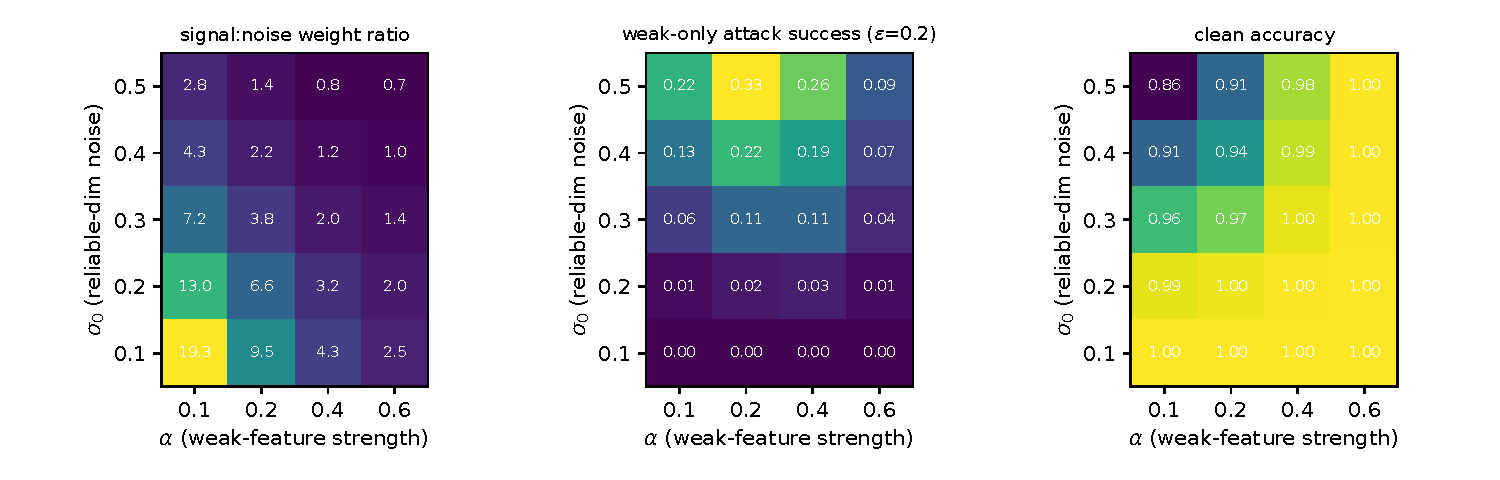
\includegraphics[width=\textwidth]{fig_fr_phase.pdf}
\caption{Weight decay $10^{-2}$. Left: reliable-to-weak weight ratio. Middle: share flipped by an attack on the weak clues alone ($\epsilon=0.2$). Right: clean accuracy.
Rows: noise of the reliable clue (lowest at the bottom); columns: strength of the weak clues.}
\label{fig:phase}
\end{figure}

\begin{itemize}
\item If the reliable clue is nearly perfect (lowest noise, bottom row), the network ignores the weak clues and the effect disappears: at the weight decay shown the weak-clue attack flips at most $0.1\%$ of points in that row, and at most about $1\%$ at any weight decay on the grid.
The network has no pressure to use clues it does not need, even though they carry information.
\item The effect grows as the reliable clue gets noisier, and peaks for moderately strong weak clues (up to $0.37$ flipped).
\item Weight decay is \emph{not} what creates the effect. Turning it up makes the network rely \emph{less} on the weak clues (for example the flipped share falls $0.25\to0.24\to0.22\to0.11$ as weight decay rises from none to the strongest value, at one setting of the grid).
\end{itemize}

\section{Does any of this happen on real images?}
\label{sec:real}

Only partly, and the honest summary is more interesting than a clean confirmation. We look at three image tasks.

\subsection{Circles and squares}

We built a small picture version of the toy world. Each $28\times28$ image shows a filled circle (label 0) or square
(label 1) on a gray background; pixel values lie in $[0,1]$. The shape \emph{is} the label (a network sees it with $99.9\%$ accuracy alone). The background gray level is only correlated with the label ($73.8\%$ accuracy alone). Noise is added to every
pixel, so the shape is hard to see by eye (Figures~\ref{fig:cleansamples}, \ref{fig:stimuli}), yet a small convolutional network reads it at $99.6\%$. (One-step attack, 10 runs.)

\begin{figure}[h]
\centering
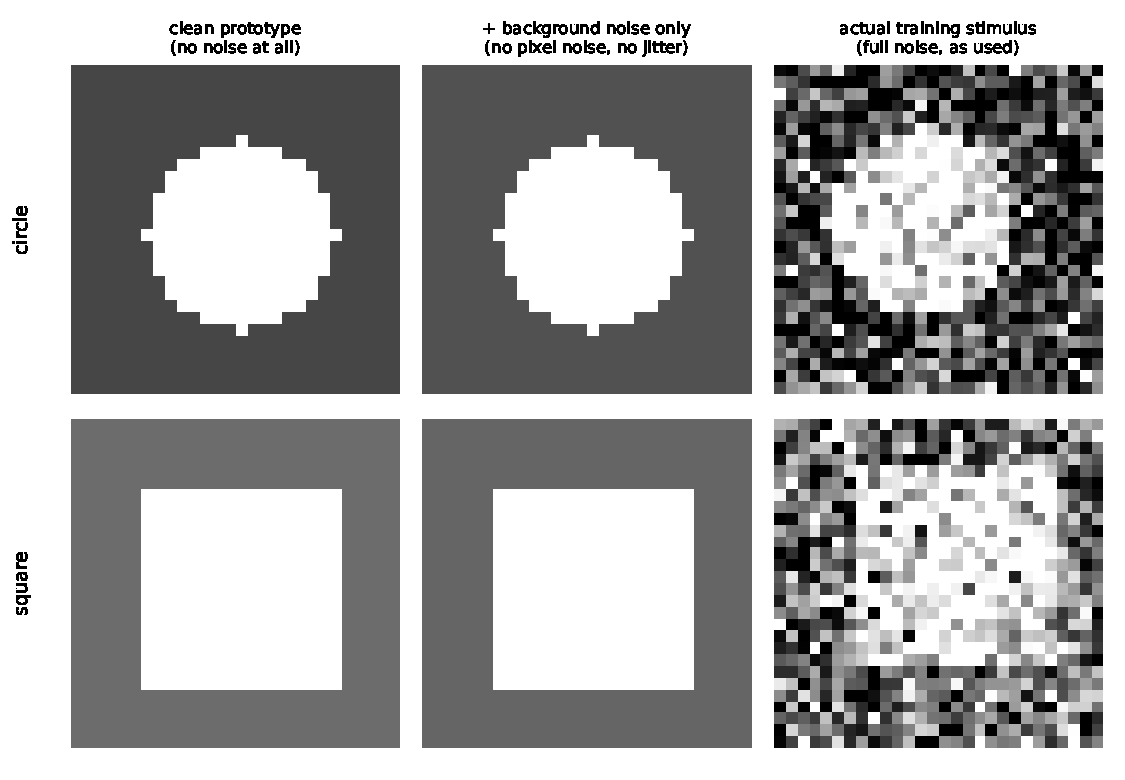
\includegraphics[width=0.74\textwidth]{fig_clean_samples.pdf}
\caption{Left: noise-free prototypes of each class (the background shade difference is visible). Middle: one sample of background-level noise. Right: an actual training image.}
\label{fig:cleansamples}
\end{figure}

\begin{figure}[h]
\centering
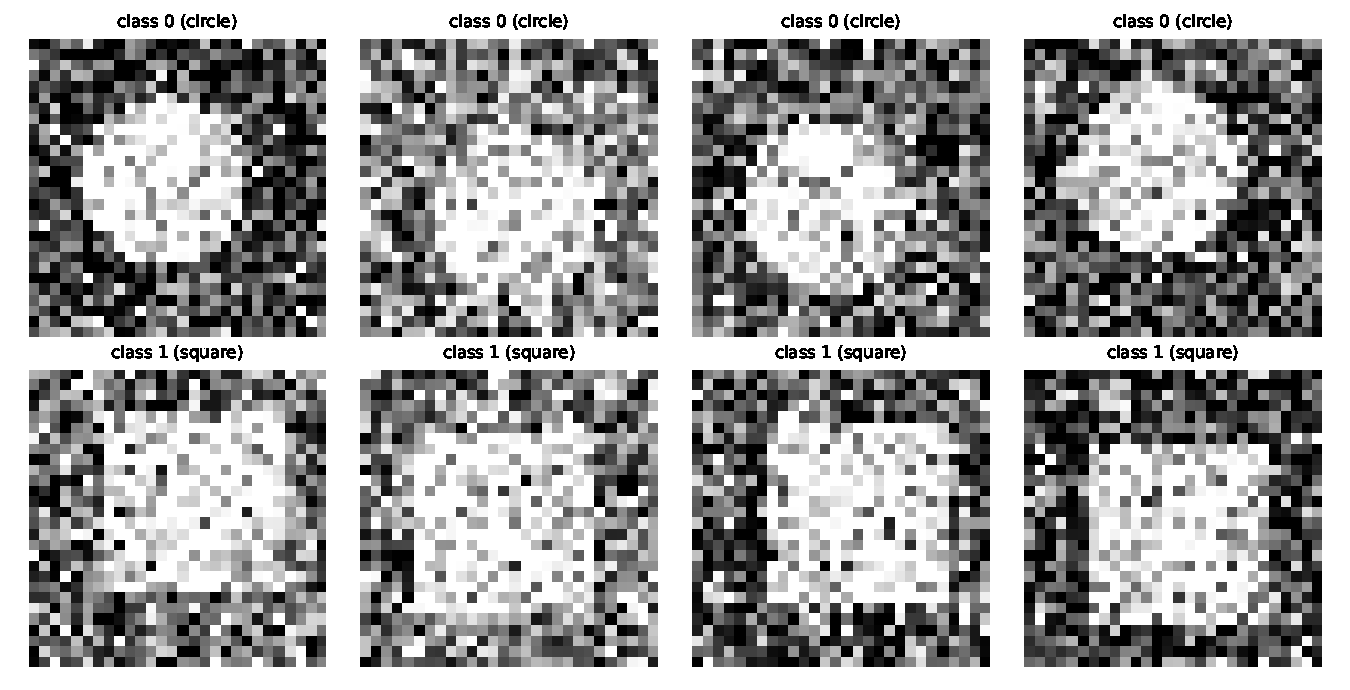
\includegraphics[width=0.82\textwidth]{fig_stimulus_examples.pdf}
\caption{Training examples. The background level varies within and across classes.}
\label{fig:stimuli}
\end{figure}

\textbf{Surprise.} In the toy task, a near-perfect reliable clue switched the effect off (Section~\ref{sec:when}). Here the shape is nearly perfect, yet the network still picks up the background: an attacker who may change \emph{only the border pixels},
never touching the shape, flips $46\%$--$71\%$ of answers at nudge sizes $0.2$--$0.4$. We do not have a full explanation; a cheap, uniform cue is easy for a convolutional network to pick up.

\begin{table}[h]
\centering
\caption{Share of image answers flipped (one-step attack), by where the attacker may change pixels (mean $\pm$ s.d.\ over 10 runs).}
\label{tab:image}
\begin{tabular}{lccc}
\toprule
nudge size & all pixels & shape region & background border \\
\midrule
0.10 & $0.942\pm0.037$ & $0.587\pm0.055$ & $0.104\pm0.076$ \\
0.20 & $1.000\pm0.000$ & $0.996\pm0.005$ & $0.464\pm0.073$ \\
0.30 & $1.000\pm0.000$ & $1.000\pm0.001$ & $0.668\pm0.082$ \\
0.40 & $1.000\pm0.000$ & $0.996\pm0.013$ & $0.711\pm0.084$ \\
\bottomrule
\end{tabular}
\end{table}

\textbf{A trap in the comparison.} The ``shape region'' column is \emph{not} the picture version of ``reliable clue only''. In the toy task, nudging the reliable clue moves one number a little. In an image the shape region
contains the shape's own pixels, and a large enough change simply redraws the shape into something else (Figure~\ref{fig:imageattack}). The shape pixels are the ground truth, not a measurement of it. So the
border-only attack is the one that matches the intended meaning of ``adversarial'': it exploits an incidental clue at a nudge too small to redraw anything.

\begin{figure}[h]
\centering
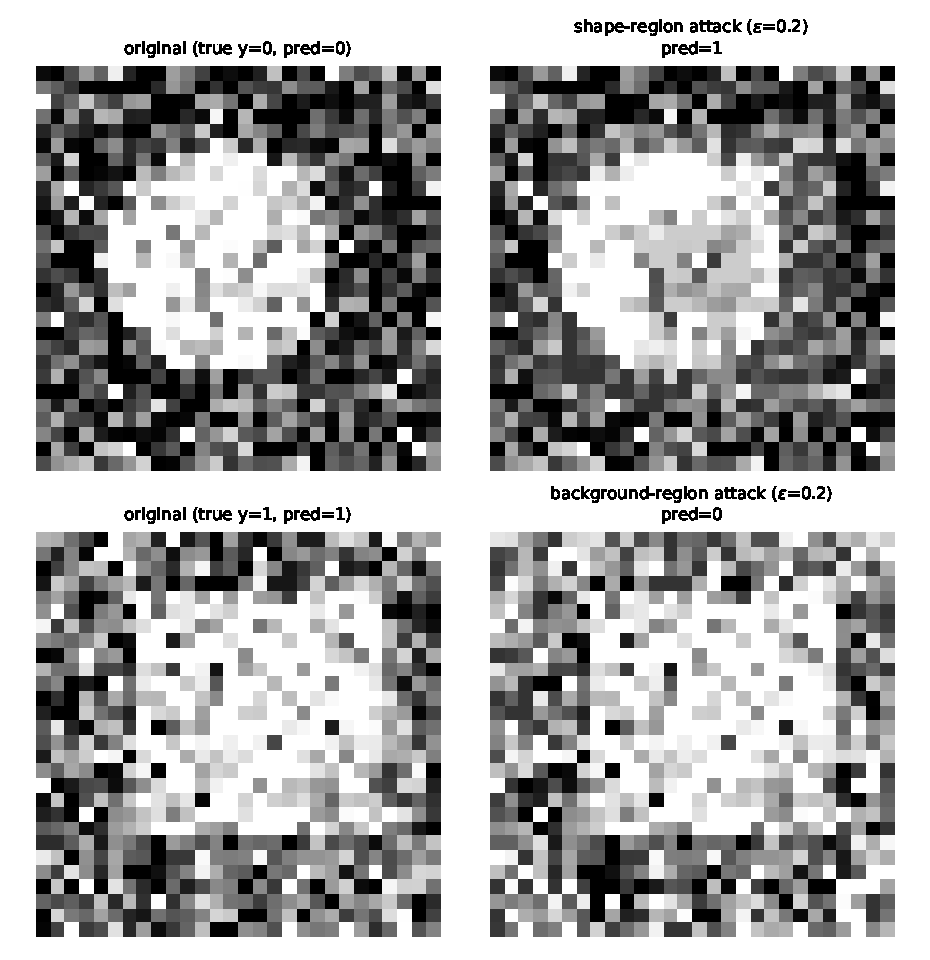
\includegraphics[width=0.58\textwidth]{fig_image_attack_example.pdf}
\caption{One run, nudge size $0.2$. Top: an attack confined to the shape region visibly distorts the shape. Bottom: an attack confined to the border changes only the background, leaves the shape untouched, and still flips the answer.}
\label{fig:imageattack}
\end{figure}

\textbf{Genuine separation helps (with a caveat).} We built a two-tower network in which one tower sees only the shape region and the other only the rest, so restricting the attack to a region restricts it to one tower's whole input. The border-tower
attack is clearly weaker than the single network's border attack ($0.312$ against $0.668$ at nudge size $0.3$; $0.454$ against $0.711$ at $0.4$) at the same accuracy ($99.7\%$), 5 runs. The shape-tower attack stays near $1.0$, as expected. We cannot
claim a clean ablation: the two-tower network has about twice the parameters and narrower connections, so some of the effect may be capacity, not separation. An iterated attack (PGD-10, 2 restarts, 5 runs) is a little stronger than the one-step attack on this task
(border attack at $0.3$: $0.654\to0.752$), but the pattern is unchanged.

\subsection{MNIST}

We scrambled the pixels of handwritten digits with a random rotation of the input space that leaves all distances and all information
unchanged, but spreads each clue over more coordinates. The straight-line size of the change needed stays the same (accuracy too), as predicted. The per-pixel flip size, however, falls by only
$12$--$14\%$, not the eightfold drop of the toy world. Digits in their ordinary pixel form are already nearly as spread out as an input can be, so there is little room left to spread.

\begin{figure}[h]
\centering
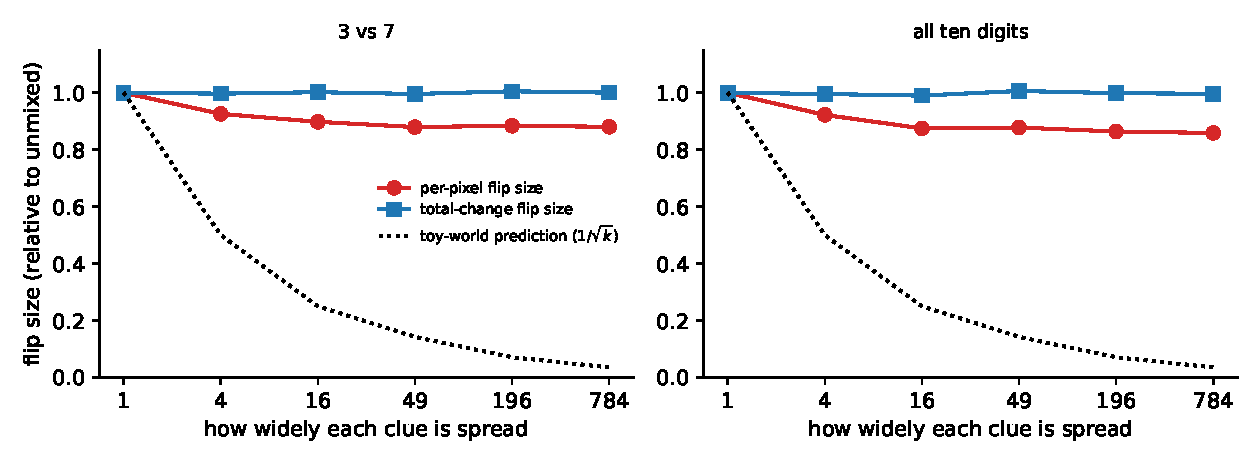
\includegraphics[width=0.9\textwidth]{fig_il_mnist_mix.pdf}
\caption{MNIST after mixing pixels within blocks of size $k$ (so each clue is spread over $k$ inputs). Blue: total-change flip size, unchanged as predicted. Red: per-pixel flip size, which drops only slightly. Dotted: what the toy world predicts ($1/\sqrt k$). Relative to $k=1$; 5 runs.}
\label{fig:mnistmix}
\end{figure}

\subsection{CIFAR-10}

We let a small image network use only the strongest $m$ patterns in the images. More patterns means higher accuracy ($44\%\to78\%$) but a $6.8\times$ smaller
per-pixel flip size. Here the loss does \emph{not} come from spreading; it comes from the model using finer, smaller-margin patterns that are individually easier to move.
(These medians are over correctly classified points, so models with few patterns are measured on an easier subset, which overstates their robustness.)

\begin{figure}[h]
\centering
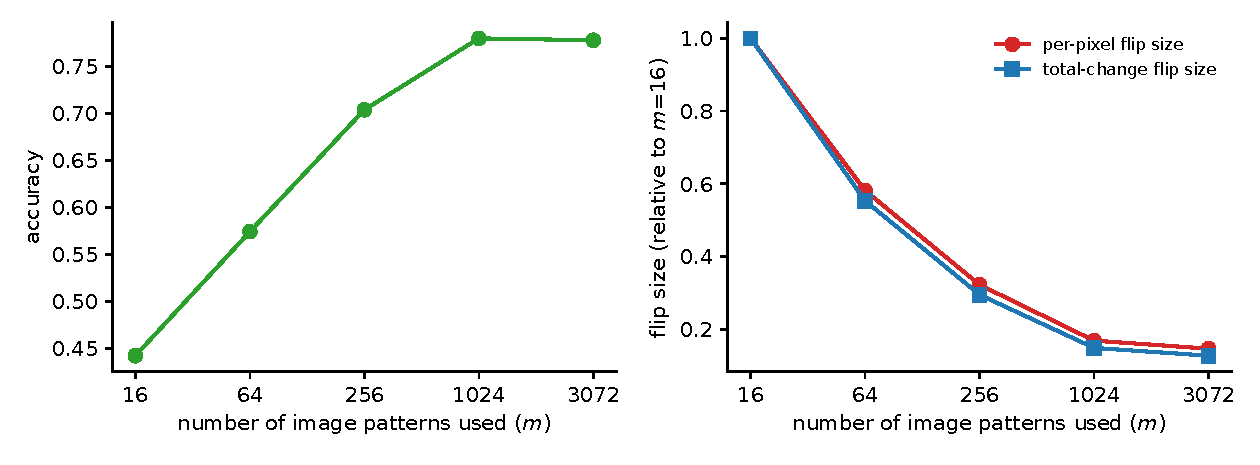
\includegraphics[width=0.9\textwidth]{fig_il_cifar_m.pdf}
\caption{CIFAR-10 with the network allowed to use only the top $m$ image patterns. Left: accuracy rises with $m$. Right: both flip sizes fall together, by about seven to eight times, so the loss is a shrinking margin, not spreading (5 runs).}
\label{fig:cifarm}
\end{figure}

\plain{The adding-up geometry is real on real images too, but natural images are already in the ``spread out'' regime, so the
toy world's eightfold effect is not what drives them. On CIFAR, the cost of using more detail is mostly smaller margins. What we have not shown: that
large deep networks on natural data work this way.}

\section{Takeaways and limits}

\begin{enumerate}
\item A network is fooled mainly because it \emph{adds up many small pieces of evidence} and the attacker may nudge all of them.
\item Weak clues are not useless, and no single weak clue is the culprit; the vulnerability is in the sum.
\item In this task it is a property of the problem and the attack rule, not a flaw in training: the best possible classifier is just as vulnerable.
\item ``Small'' (relative to the nudge), not ``unreliable'', is what makes a clue fragile.
\item Fixes work by throwing away information, and cost accuracy; switching whole inputs off works better than shrinking everything, and concentrating on one clue creates a new single point of failure.
\item Sparsity of the \emph{weights} helps; sparsity of the \emph{activity} does not, and breaks networks all at once.
\item Always judge the nudge against the size of the clue, and beware near-perfect clues, which can hide the effect entirely.
\end{enumerate}

\paragraph{Limits.} One toy task with independent clues, a single small network, and a one-step attack in the main comparisons. The real-data checks
support the geometry but not the toy world's size of effect. We did not test correlated clues, deep networks, or adversarial training.

\paragraph{Where to go next.} A natural extension is to ask whether a network whose internal representation is \emph{equivariant} to a physical transformation (rotation, scale, viewpoint) makes attacks transfer
predictably across viewpoints, since by the chain rule the gradient, and so an attack built from it, would then transform predictably too. The toy world gives a controlled place to start; we have not tested this here.

\appendix

\section{Experimental details}
\label{app:details}

\paragraph{Toy task.} Given the label $y$, each input is an independent bell-curve variable with mean $(y-\tfrac12)\Delta\mu_i$ and standard deviation $\sigma_i$, no clipping. Reliable clue: $\Delta\mu=1.0$, $\sigma=0.3$.
Weak clues: $\Delta\mu=0.4$, $\sigma=0.25$. The best possible rule is a weighted sum with weights $\Delta\mu_i/\sigma_i^2$ ($11.1$ and $6.4$) and is exact. Single-clue accuracy is $\Phi(\Delta\mu/2\sigma)$.

\paragraph{Networks and training.} One hidden layer of 8 ReLU units, two outputs; Adam (learning rate $0.02$), 500 full-batch steps, weight decay $10^{-2}$ unless varied; 4{,}000 training and 1{,}000 test points (2{,}000 test points for
the flip-size experiments). Each of the 10 runs reseeds the data and the initialisation. Quantities are reported as mean $\pm$ one sample standard deviation across runs. Model C's leftover weights are scaled before training (they receive no gradient, so they stay at that scale).

\paragraph{Attacks.} ``Flipped'' is the share of correctly classified test points whose predicted label changes after the one-step attack (nudge $\epsilon$ times the sign of the loss gradient, optionally masked to a subset of inputs).
``Flip size'' is the smallest nudge that flips a given point: computed exactly for the best possible rule ($|\text{LLR}|/\|w\|_1$ per input, or $|\text{LLR}|/\|w\|_2$ for straight-line distance) and by per-point bisection over a 20-step attack for trained networks (14 bisection steps).
The tables report the median flip size over points, then average over runs.

\paragraph{Spread experiment.} Total discriminability $d'=1/0.3$ (accuracy $95\%$) split equally over $k\in\{1,2,4,\ldots,64\}$ inputs, each with noise $0.25$; a network is trained at each $k$ ($10$ runs).
\textbf{Size-versus-reliability experiment:} one input with class gap $\Delta\mu\in\{0.05,\ldots,0.8\}$ and reliability $d'\in\{1.5,3,6\}$ (noise $\Delta\mu/d'$), with a fixed standardising layer so tiny inputs are not handicapped by the optimiser; attacks act on the raw input.

\paragraph{Regularisers.} $L_1$ and group Lasso penalties act on the first-layer weights with no other weight decay (group Lasso: one norm per input column); elastic net uses $L_1=0.1$ with the $L_2$ strength varied; pruning zeros the smallest-norm weak columns after ordinary training with no retraining. The activity penalty adds
$\lambda$ times the mean hidden activation. A run counts as a dead network if its test accuracy is below $0.6$.

\paragraph{Phase diagram.} Reliable-clue noise $\in\{0.1,\ldots,0.5\}$, weak-clue gap $\in\{0.1,0.2,0.4,0.6\}$, weight decay $\in\{0,10^{-3},10^{-2},10^{-1}\}$; 5 runs per cell; attack size $0.2$.

\paragraph{Images.} Circles and squares: $28\times28$ grayscale, shape position jittered by $\pm2$ pixels, background level shifted by class with overlapping noise, plus per-pixel noise; a two-layer convolutional network; 10 runs (5 for the two-tower network and the iterated-attack check).
Figure~\ref{fig:mnistadv} uses the unmixed MNIST network below, with the smallest of the nudge sizes $0.02$--$0.08$ at which an iterated attack flips the answer. MNIST: a 784--256--10 network trained with momentum SGD on 10{,}000 images, 1{,}000 test images, 5 runs, inputs rotated within random blocks of size $k\in\{1,4,16,49,196,784\}$. CIFAR-10: a five-layer convolutional network on the top-$m$ principal components
($m\in\{16,64,256,1024,3072\}$) of the images; 20{,}000 training and 500 test images, 5 runs; the attacker perturbs raw pixels with no clipping. Code for all experiments accompanies this paper.

\section{Glossary}
\label{sec:glossary}

\begin{description}
\item[Adversarial example] An input changed slightly, on purpose, so that a model gets it wrong.
\item[Clue / feature] A number the model reads. \emph{Reliable} if it alone predicts the label well; \emph{weak} if not; \emph{small} if its two class averages are close
compared with the allowed nudge.
\item[Nudge size $\epsilon$] The most the attacker may change each input.
\item[Flip size] The smallest nudge size at which a given answer flips.
\item[Best possible (Bayes-optimal) classifier] The rule with the highest achievable accuracy given how the data were generated.
\item[$L_1$, group Lasso, $L_2$] Training penalties on the model's weights. $L_1$ and group Lasso push whole inputs to zero; $L_2$ ordinary weight decay shrinks everything.
\end{description}

\begin{thebibliography}{9}

\bibitem{szegedy2014}
C.~Szegedy, W.~Zaremba, I.~Sutskever, J.~Bruna, D.~Erhan, I.~Goodfellow, R.~Fergus.
\emph{Intriguing properties of neural networks}. ICLR, 2014.

\bibitem{goodfellow2015}
I.~Goodfellow, J.~Shlens, C.~Szegedy.
\emph{Explaining and Harnessing Adversarial Examples}. ICLR, 2015.

\bibitem{madry2018}
A.~Madry, A.~Makelov, L.~Schmidt, D.~Tsipras, A.~Vladu.
\emph{Towards Deep Learning Models Resistant to Adversarial Attacks}. ICLR, 2018.

\bibitem{athalye2018}
A.~Athalye, N.~Carlini, D.~Wagner.
\emph{Obfuscated Gradients Give a False Sense of Security: Circumventing Defenses to Adversarial Examples}. ICML, 2018.

\bibitem{tsipras2018}
D.~Tsipras, S.~Santurkar, L.~Engstrom, A.~Turner, A.~Madry.
\emph{Robustness May Be at Odds with Accuracy}. ICLR, 2019.

\bibitem{ilyas2019}
A.~Ilyas, S.~Santurkar, D.~Tsipras, L.~Engstrom, B.~Tran, A.~Madry.
\emph{Adversarial Examples Are Not Bugs, They Are Features}. NeurIPS, 2019.

\end{thebibliography}

\end{document}
